\chapter{Graphing Commands}\label{s:plot}

R, and thus Zelig, can produce exceptionally beautiful plots.  Many
built-in plotting functions exist, including scatter plots, line
charts, histograms, bar charts, pie charts, ternary diagrams, contour
plots, and a variety of three-dimensional graphs.  If you desire, you
can exercise a high degree of control to generate just the right
graphic.  Zelig includes several default plots for one-observation
simulations for each model.  To view these plots on-screen, simply
type {\tt plot(s.out)}, where {\tt s.out} is the output from {\tt
  sim()}.  Depending on the model chosen, {\tt plot()} will return
different plots.

If you wish to create your own plots, this section reviews the most
basic procedures for creating and saving two-dimensional plots.  R
plots material in two steps:  
\begin{enumerate}
\item You must call an output device (discussed in \Sref{ss:output}),
  select a type of plot, draw a plotting region, draw axes, and plot
  the given data.  At this stage, you may also define axes labels, the
  plot title, and colors for the plotted data.  Step one is described
  in \Sref{ss:draw} below.
\item Optionally, you may add points, lines, text, or a legend to the
  existing plot.  These commands are described in \Sref{ss:add}.
\end{enumerate}

\section{Drawing Plots}\label{ss:draw}

The most generic plotting command is \texttt{plot()}, which
automatically recognizes the type of R object(s) you are trying to
plot and selects the best type of plot.  The most common graphs
returned by \texttt{plot()} are as follows:
\begin{enumerate}
\item If \texttt{X} is a variable of length $n$, \texttt{plot(X)}
  returns a scatter plot of $(x_i, i)$ for $i = 1, \dots n$.  If X is
  unsorted, this procedure produces a messy graph.  Use
  \texttt{plot(sort(X))} to arrange the plotted values of $(x_i, i)$
  from smallest to largest.
\item With two numeric vectors \texttt{X} and \texttt{Y}, both of
  length $n$, \texttt{plot(X, Y)} plots a scatter plot of each point
  $(x_i, y_i)$ for $i = 1, \dots n$.  Alternatively, if Z is an object
  with two vectors, \texttt{plot(Z)} also creates a scatter plot.
\end{enumerate}

Optional arguments specific to \texttt{plot} include:
\begin{itemize}
\item \texttt{main} creates a title for the graph, and \texttt{xlab}
  and \texttt{ylab} label the x and y axes, respectively. For
  example,
\begin{verbatim}
plot(x, y, main = "My Lovely Plot", xlab = "Explanatory Variable", 
     ylab = "Dependent Variable")
\end{verbatim}
  
\item \texttt{type} controls the type of plot you request.  The
  default is \texttt{plot(x, y, type = "p")}, but you may choose among
  the following types:
    \begin{table}[!h]
    \begin{quote}
    \begin{tabular}{cl}
    {\tt "p"} & points\\
    {\tt "l"} & lines\\
    {\tt "b"} & both points and lines\\
    {\tt "c"} & lines drawn up to but not including the points\\
    {\tt "h"} & histogram\\
    {\tt "s"} & a step function\\
    {\tt "n"} & a blank plotting region ( with the axes specified)
    \end{tabular}
    \end{quote}
    \end{table}
\item If you choose {\tt type = "p"}, R plots open circles by default.
  You can change the type of point by specifying the {\tt pch}
  argument.  For example, \texttt{plot(x, y, type = "p", pch = 19)}
  creates a scatter-plot of filled circles.  Other options for {\tt
    pch} include:
    \begin{table}[!h]
    \begin{quote}
    \begin{tabular}{cl}
    19 & solid circle (a disk) \\
    20 & smaller solid circle \\
    21 & circle\\
    22 & square\\
    23 & diamond \\
    24 & triangle pointed up\\
    25 & triangle pointed down\\
    \end{tabular}
    \end{quote}
    \end{table}

In addition, you can specify your own symbols by using, for example,
{\tt pch = "*"} or {\tt pch = "."}.  

\item If you choose {\tt type = "l"}, R plots solid lines by default.
  Use the optional {\tt lty} argument to set the line type.  For
  example, {\tt plot(x, y, type = "l", lty = "dashed")} plots a dashed
  line.  Other options are dotted, dotdash, longdash, and twodash.
  
\item \texttt{col} sets the color of the points, lines, or bars.  For
  example, \texttt{plot(x, y, type = "b", pch = 20, lty = "dotted",
    col = "violet")} plots small circles connected by a dotted line,
  both of which are violet.  (The axes and labels remain black.)  Use
  \texttt{colors()} to see the full list of available colors.
  
\item \texttt{xlim} and {\tt ylim} set the limits to the $x$-axis and
  $y$-axis.  For example, \texttt{plot(x, y, xlim = c(0, 25), ylim =
    c(-15, 5))} sets range of the $x$-axis to [0, 25] and the range of
  the $y$-axis to $[-15, 5]$.
\end{itemize}
For additional plotting options, refer to {\tt help(par)}.

\section{Adding Points, Lines, and Legends to Existing Plots}\label{ss:add}

Once you have created a plot, you can \emph{add} points, lines, text,
or a legend.  To place each of these elements, R uses coordinates
defined in terms of the x-axes and y-axes of the plot area, not
coordinates defined in terms of the the plotting window or device.
For example, if your plot has an x-axis with values between $[0,
100]$, and a y-axis with values between $[50, 75]$, you may add a
point at $(55,55)$.  

\begin{itemize}
\item \textbf{points()} plots one or more sets of points.  Use
  \texttt{pch} with \texttt{points} to add points to an existing plot.
  For example, \texttt{points(P, Q, pch = ".", col = "forest green")}
  plots each $(p_i, q_i)$ as tiny green dots.
\item \textbf{lines()} joins the specified points with line segments.
  The arguments \texttt{col} and \texttt{lty} may also be used.  For
  example, \texttt{lines(X, Y, col = "blue", lty = "dotted")} draws a
  blue dotted line from each set of points $(x_i, y_i)$ to the next.
  Alternatively, \texttt{lines} also takes command output which
  specifies $(x, y)$ coordinates.  For example, \texttt{density(Z)}
  creates a vector of $x$ and a vector of $y$, and {\tt
    plot(density(Z))} draws the kernel density function.  
\item \textbf{text()} adds a character string at the specified set of
  $(x,y)$ coordinates.  For example, {\tt text(5, 5, labels = "Key
    Point")} adds the label ``Key Point'' at the plot location
  $(5,5)$.  You may also choose the font using the {\tt font} option,
  the size of the font relative to the axis labels using the {\tt cex}
  option, and choose a color using the {\tt col} option.  The full
  list of options may be accessed using {\tt help(text)}.   
\item \textbf{legend()} places a legend at a specified set of $(x,y)$
  coordinates.  Type {\tt demo(vertci)} to see an example for {\tt
    legend()}.  
\end{itemize}

\section{Saving Graphs to Files}\label{ss:output}

By default, R displays graphs in a window on your screen.  To save R
plots to file (to include them in a paper, for example), preface your
plotting commands with:
\begin{verbatim}
> ps.options(family = c("Times"), pointsize = 12)
> postscript(file = "mygraph.eps", horizontal = FALSE, paper = "special",
             width = 6.25, height = 4)
\end{verbatim}
where the \texttt{ps.options()} command sets the font type and size in
the output file, and the \texttt{postscript} command allows you to
specify the name of the file as well as several additional options.
Using {\tt paper = special} allows you to specify the width and height
of the encapsulated postscript region in inches (6.25 inches long and
4 inches high, in this case), and the statement \texttt{horizontal =
  FALSE} suppresses R's default landscape orientation.  Alternatively,
you may use {\tt pdf()} instead of {\tt postscript()}.  If you wish to
select postscript options for .pdf output, you may do so using options
in {\tt pdf()}.  For example:
\begin{verbatim}
> pdf(file = "mygraph.pdf", width = 6.25, height = 4, family = "Times", 
+     pointsize = 12)
\end{verbatim}

At the end of every plot, you should close your output device.  The
command \texttt{dev.off()} stops writing and saves the \texttt{.eps}
or {\tt .pdf} file to your working directory.  If you forget to close
the file, you will write all subsequent plots to the same file,
overwriting previous plots.  You may also use \texttt{dev.off()} to close
on-screen plot windows.

To write multiple plots to the same file, you can use the following
options:  
\begin{itemize}
\item For plots on separate pages in the same {\tt .pdf} document, use
\begin{verbatim}
> pdf(file = "mygraph.pdf", width = 6.25, height = 4, family = "Times", 
+     pointsize = 12, onefile = TRUE)
\end{verbatim}
\item For multiple plots on one page, initialize either a {\tt .pdf}
or {\tt .eps} file, then (before any plotting commands) type:  
\begin{verbatim}
par(mfrow = c(2, 4))
\end{verbatim}
This creates a grid that has two rows and four columns.  Your plot
statements will populate the grid going across the first row, then the
second row, from left to right.  
\end{itemize}

\newpage

\section{Examples}

\subsection{Descriptive Plots: Box-plots}

\begin{center}
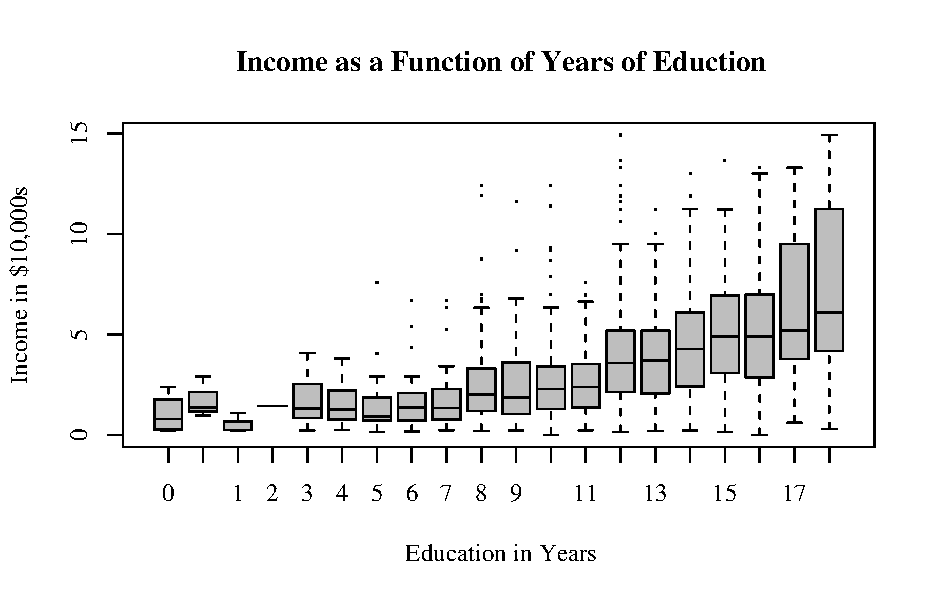
\includegraphics{figs/sample1}
\end{center}
Using the sample \texttt{turnout} data set included with Zelig, the
following commands will produce the graph above.
\begin{verbatim}
> library(Zelig)                             # Loads the Zelig package.
> data (turnout)                             # Loads the sample data.
> boxplot(income ~ educate,                  # Creates a boxplot with income
+  data = turnout, col = "grey", pch = ".",  #  as a function of education.  
+  main = "Income as a Function of Years of Education", 
+  xlab = "Education in Years", ylab = "Income in \$10,000s")
\end{verbatim}

\newpage

\subsection{Density Plots: A Histogram}

Histograms are easy ways to evaluate the density of a quantity of
interest.  

\begin{center}
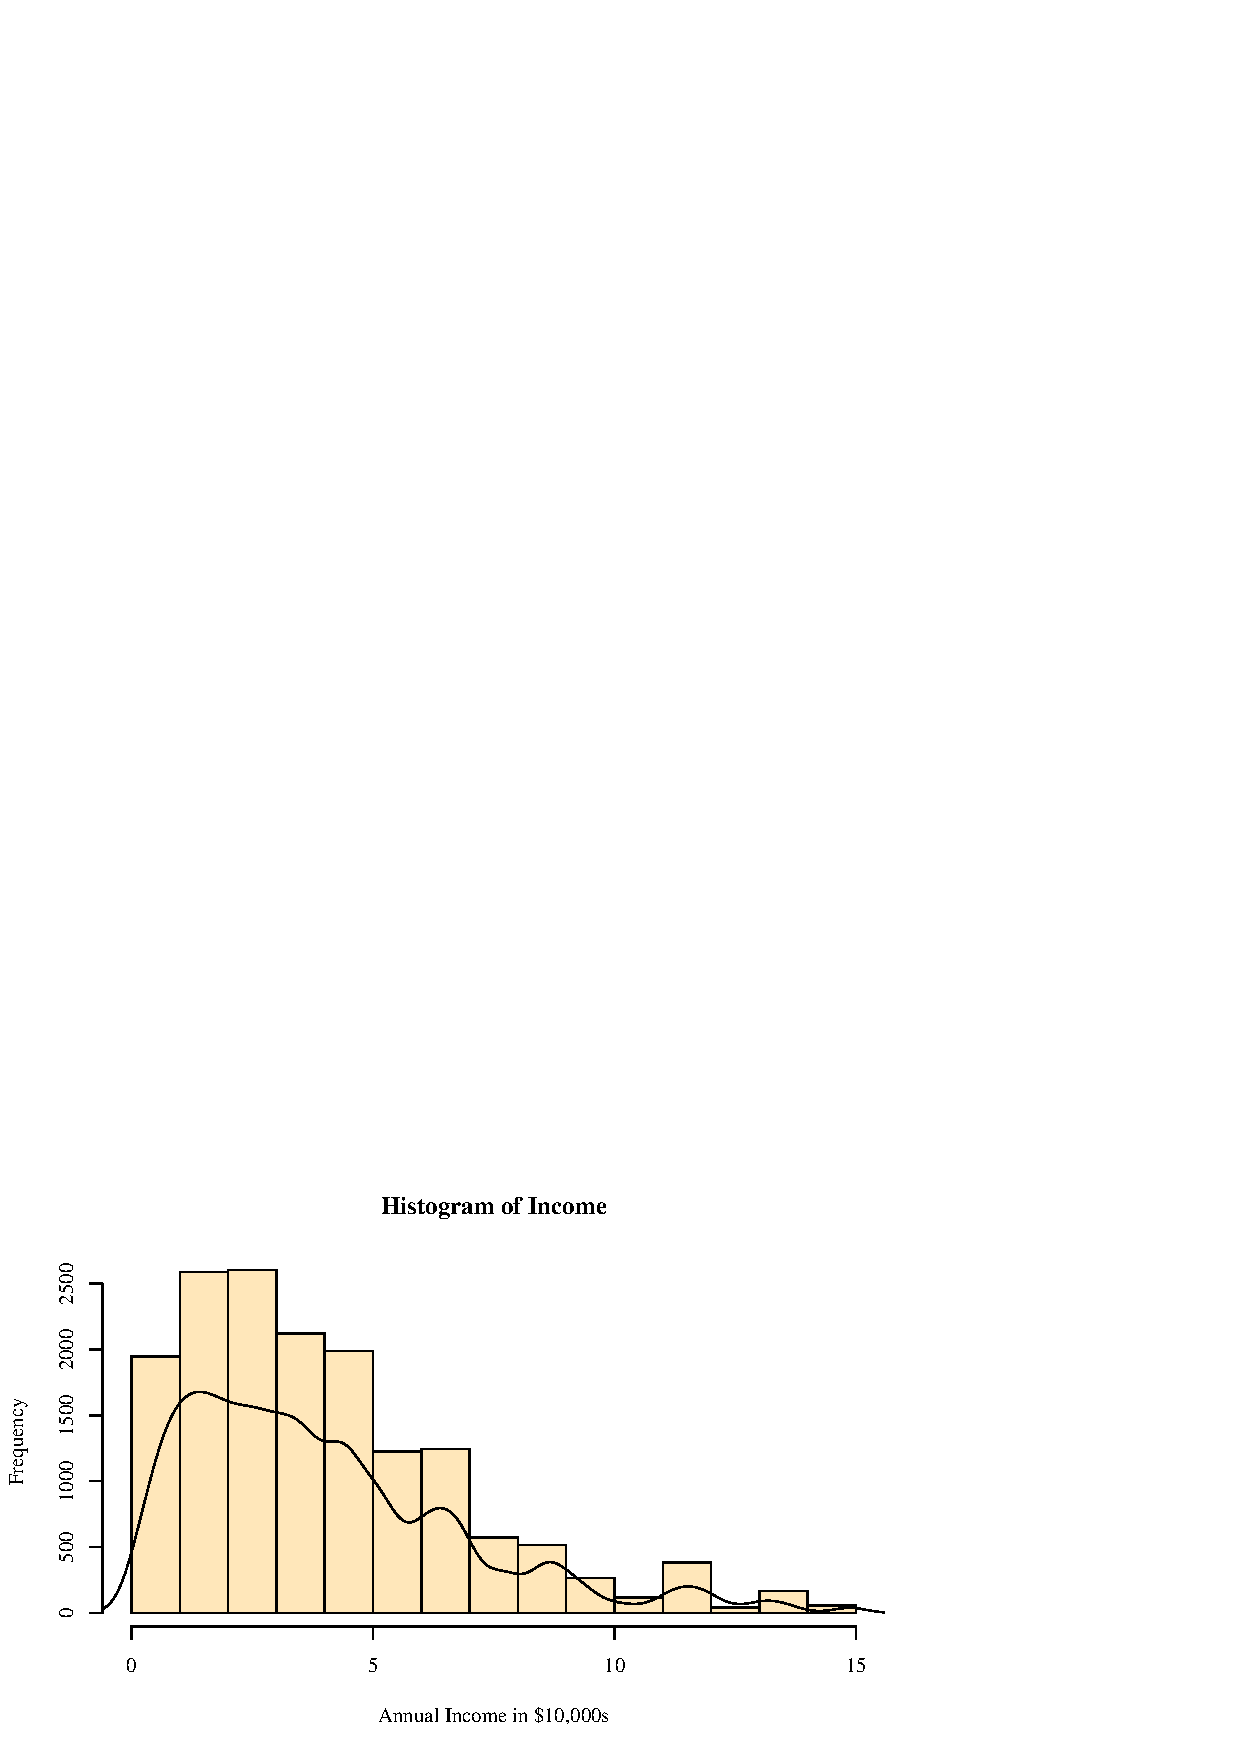
\includegraphics{figs/sample2}
\end{center}

Here's the code to create this graph:
\begin{verbatim}
> library(Zelig)                              # Loads the Zelig package.
> data(turnout)                               # Loads the sample data set.
> truehist(turnout$income,  col = "wheat1",   # Calls the main plot, with   
+      xlab = "Annual Income in $10,000s",    #  options.  
+      main = "Histogram of Income") 
> lines(density(turnout$income))              # Adds the kernel density line.  
\end{verbatim} %$

\newpage

\subsection{Advanced Examples} 

The examples above are simple examples which only skim the surface of
R's plotting potential.  We include more advanced, model-specific
plots in the Zelig demo scripts, and have created functions that
automate some of these plots, including:  

\begin{enumerate}
  
\item {\bf Ternary Diagrams} describe the predicted probability of a
  categorical dependent variable that has three observed outcomes.
  You may choose to use this plot with the multinomial logit, the
  ordinal logit, or the ordinal probit models (Katz and King,
  1999).\nocite{KatKin99} See \Sref{ternary} for the sample code, type
  {\tt demo(mlogit)} at the R prompt to run the example, and refer to
  Section \ref{ternary} to add points to a ternary diagram.
  
\begin{center}
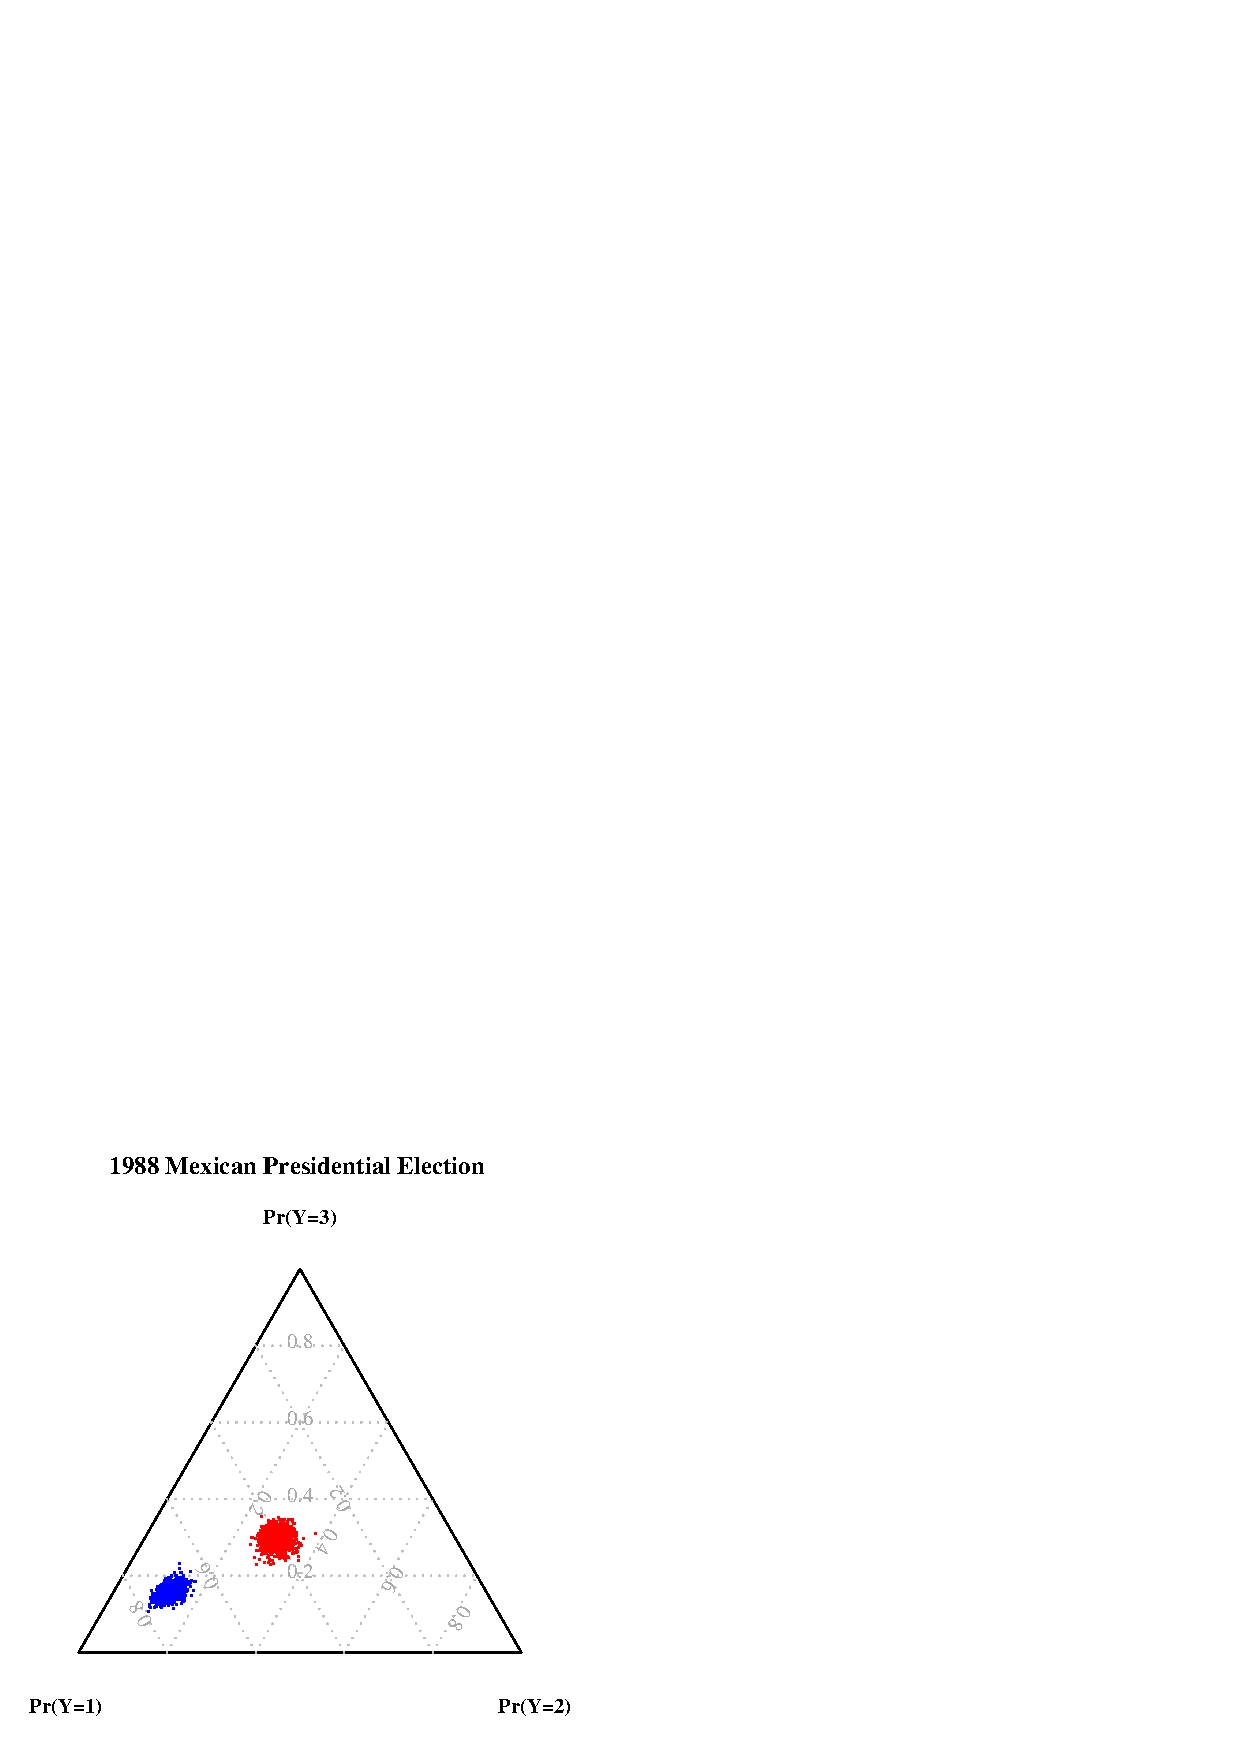
\includegraphics{figs/ternary}
\end{center}

\newpage

\item {\bf ROC Plots} summarize how well models for binary dependent
  variables (logit, probit, and relogit) fit the data.  The ROC plot
  evaluates the fraction of 0's and 1's correctly predicted for every
  possible threshold value at which the continuous Prob$(Y = 1)$ may
  be realized as a dichotomous prediction.  The closer the ROC curve
  is to the upper right corner of the plot, the better the fit of the
  model specification (King and Zeng, 2002\emph{b})\nocite{KinZen02}.
  See Section \ref{ROC} for the sample code, and type {\tt demo(roc)} at the
  R prompt to run the example.

\begin{center}
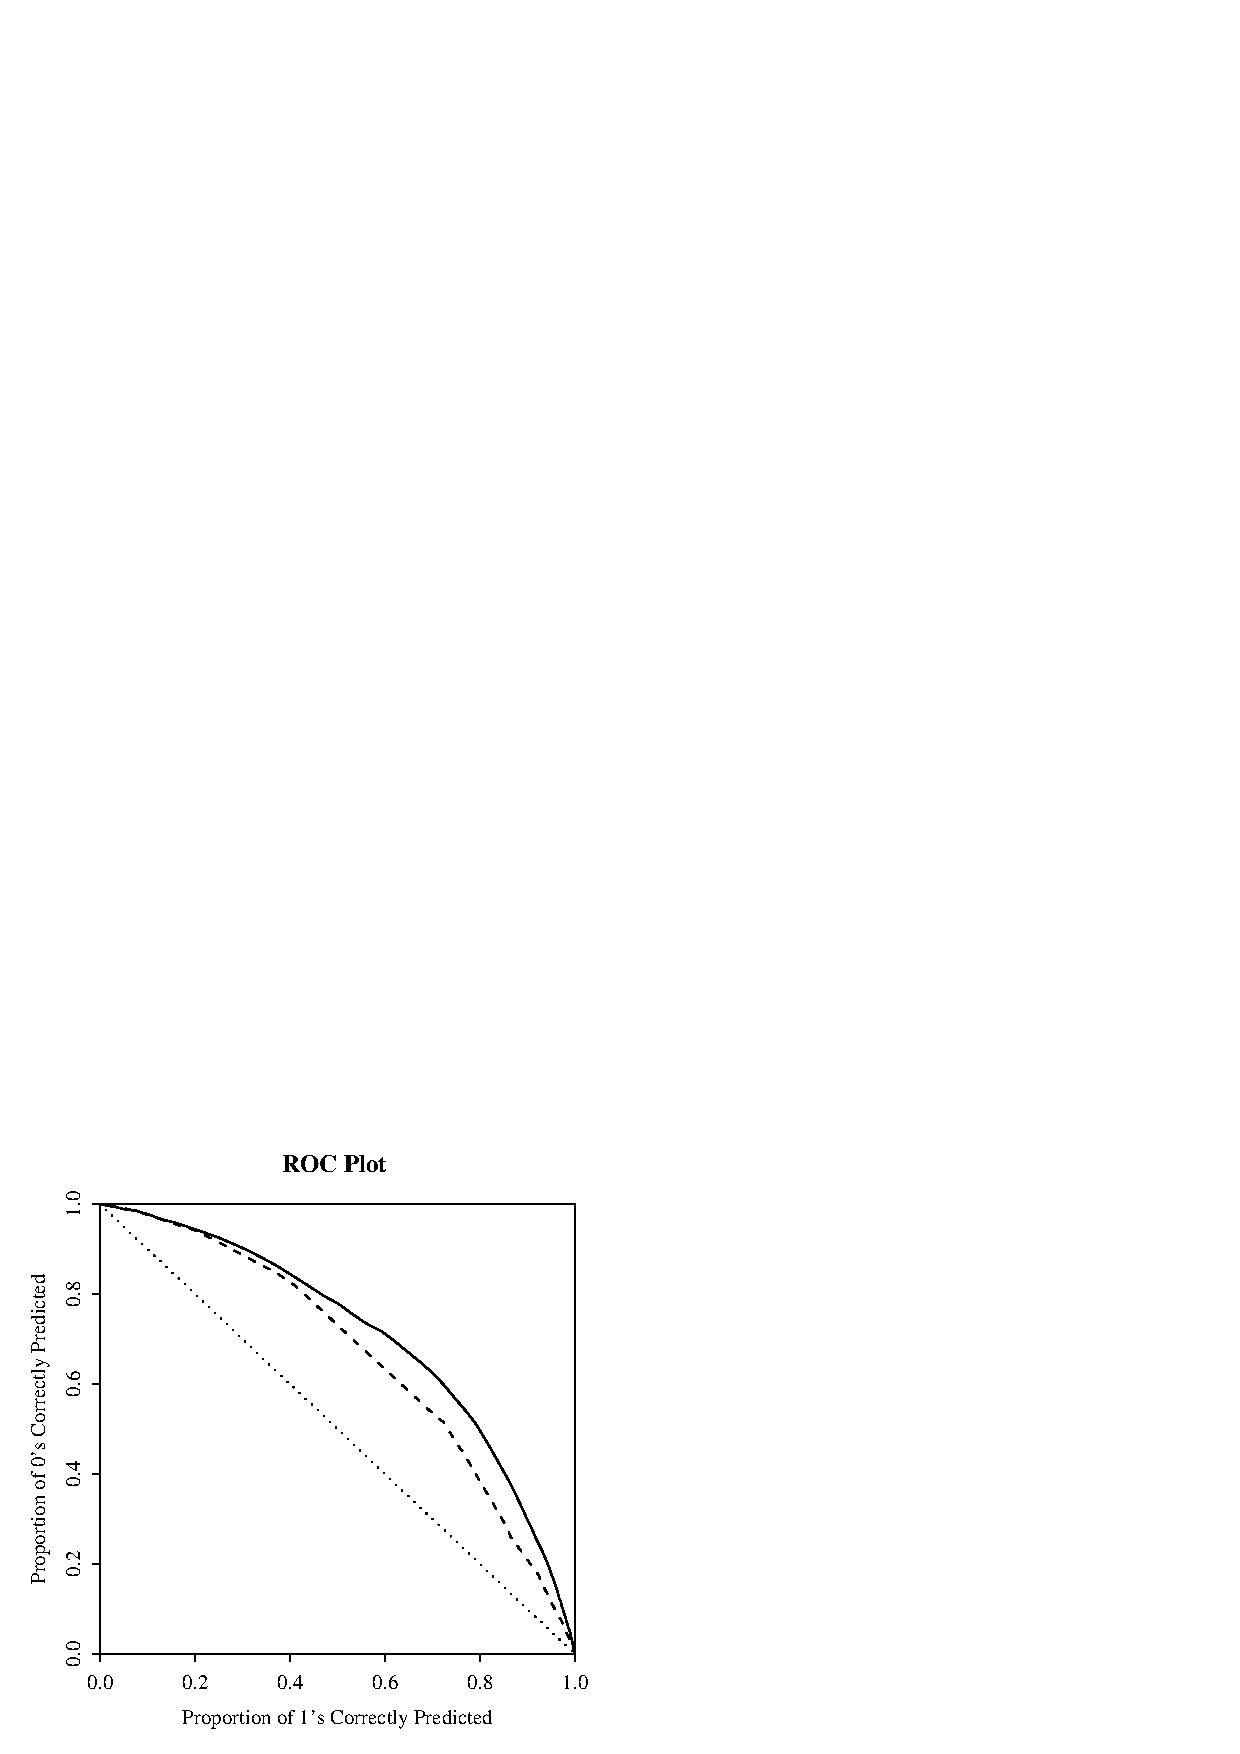
\includegraphics{figs/roc}
\end{center}

\newpage

\item {\bf Vertical Confidence Intervals} may be used for almost any
  model, and describe simulated confidence intervals for any quantity
  of interest while allowing one of the explanatory variables to vary
  over a given range of values (King, Tomz and Wittenberg,
  2000)\nocite{KinTomWit00}. Type {\tt demo(vertci)} at the R prompt to
  run the example, and {\tt help.zelig(plot.ci)} for the manual page.

\begin{center}
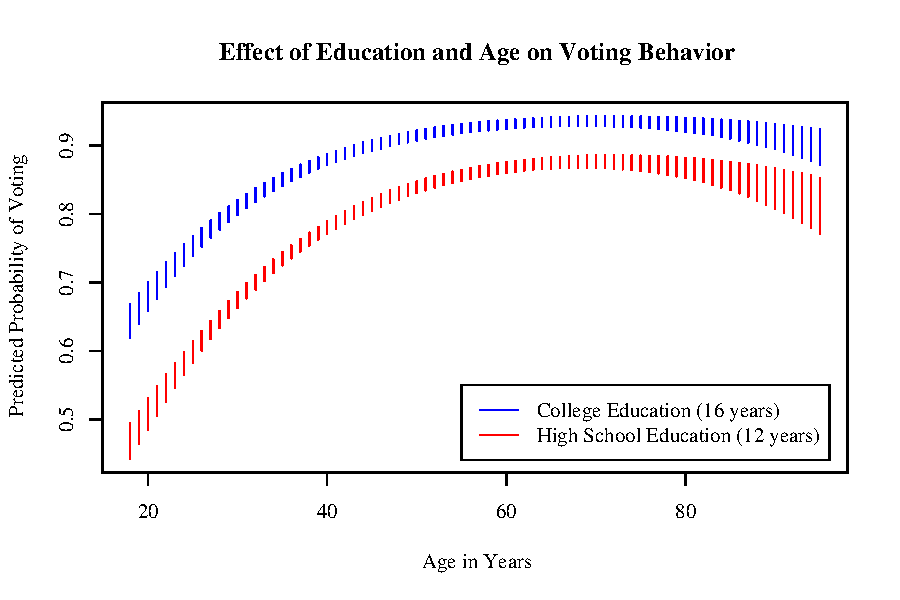
\includegraphics{figs/vertci}
\label{plot.vertci}
\end{center}

\end{enumerate}

%%% Local Variables: 
%%% mode: LaTeX
%%% TeX-master: "zelig"
%%% End:

